\chapter{Introduction}
\label{chap:intro}
\chapterquote{Confusion is the natural  state of the mathematician.}{Lior Silberman}

\chapterquote{What if I slept a little more and forgot about all this nonsense.}{Franz Kafka}


This thesis is concerned with uniting two fundamental mathematical objects: the graph and the simplex. A graph is fundamentally a  \emph{combinatorial} object---it can be described purely by means of finite sets and must not refer to any underlying geometric space.  
Simplices, on  the other hand, are inherently  geometric. As essentially high dimensional triangles, any complete description of a simplex must include certain geometric information; the distance between its vertices, for example. Thus, a simplex cannot be divorced from an  underlying metric space. 

The pessimistic reader may interject that graphs can \emph{of course} be viewed geometrically. For instance, he or she continues, it  is well-known that the shortest path between two vertices constitutes  a metric on  the graph. We in turn interrupt the interrupter and remark that while graphs \emph{can} be  given  geometric interpretations, it is \emph{not necessary} that  they are. Indeed, a graph can  be described by two finite lists: a list of its vertices and a second of the connections between these vertices (perhaps with  weights  given  to the  edges). No underlying geometric space need be defined. 

Due  to the combinatorial  nature of the graph and the geometric nature of the simplex, a connection between the two objects might seem unlikely a  priori. It is precisely this fact which makes such a connection worth studying. 
The original  link  between graphs and simplices was uncovered by 
Miroslav Fiedler  in his 1993 paper entitled ``A geometric approach to the Laplacian matrix of a graph"~\cite{fiedler1993geometric}. Here he introduced the machinery needed to define the central  object in what we will henceforth refer to as the \emph{graph-simplex correspondence}: a bijection between connected, weighted graphs and hyperacute simplices. As we will see,  however, this bijection is not the only mapping between graphs and simplices. Indeed,  this  thesis will concern itself with four mappings  between graphs and simplices. 

Unfortunately (we believe) for  the mathematical community,  Fiedler's investigations in this area  has  gone relatively unnoticed. Convinced as we are of  the beauty and  utility of such  work, this dissertation aims to present Fiedler's  results in a concise, clarifying, and self-contained fashion,  expand on the mathematical  foundations of the correspondence, and explore new applications thereof. Our primary motivation is to convince the reader that the graph-simplex correspondence is a  useful tool for studying both graphs and simplices,  and  can shed light on various  aspects of both of these objects which are  overlooked by other  methods. Given the ubiquity of graphs in the mathematical  sciences, both in theory and in application, the possibility of a new tool with which to analyze and interpret holds possibly vast promise. 



\section{Prior Work}
\label{sec:intro_prior_work}


As we stated  above, Miroslav Fiedler was the ``primary  mover''  in  uncovering the graph-simplex correspondence~\cite{fiedler1993geometric,fiedler2005geometry,fiedler2011matrices}.  This work was remained largely unnoticed until very recently, when Devriendt and Van Mieghem used the geometry of the graph as intuition behind investigating  a graph's ``best conducting node''~\cite{van2017pseudoinverse} and  then provided a summary  of Fiedler's results~\cite{devriendt2018simplex}. All of this work is concerned  with a connected and possibly  weighted graph $G$ and what we will henceforth  refer to as its  \emph{combinatorial simplices}, $\splx_G$ and $\splx_G^+$. (This is in contrast its \emph{normalized simplices}, which we  will define and explore later.) 

Fiedler uncovered  the graph-simplex correspondence by means of  a more general  relationship between matrices and simplices.  In particular, he associated with each symmetric matrix $\Q$ whose range space is orthogonal to the all ones vector (i.e.,  $\Q\one=\zero$) a unique (up to congruence) hyperacute simplex. Since the Laplacian  matrix  $\L_G$ of a connected, weighted graph  $G$ obeys this constraint, this associates with  each such graph a hyperacute simplex  $\splx_G^+$.   
For  reasons which will become clear later, we call $\splx_G^+$ the \emph{inverse} (combinatorial) simplex of $G$. 
Fiedler associated $\L_G$ and $\splx_G^+$  by means of a matrix equation which involved several somewhat complex components, including  the gram matrix of the outer normals of the simplex and  the radius of its circumscribed ellipsoid. While this matrix representation is useful for various reasons---elaborated upon in  Section~\ref{sec:block_matrix}---the correspondence can  be simplified  by means of working solely  with the Graph's Laplacian  matrix. This is the approach  recently taken by Devriendt  and  Van  Mieghem~\cite{devriendt2018simplex}. They simplify and summarize Fiedler's main  results and focus mainly on one  side of the correspondence---namely,  given $G$,  they examine  the properties of  its associated  simplices $\splx_G$ and $\splx_G^+$. 
Devriendt and  Van Mieghem also make explicit the connection between a graph's (combinatorial) simplex, $\splx_G$, and  its  inverse  simplex, $\splx_G^+$. While Fiedler was aware  of the existence of  $\splx_G$---he later examines the properties of its circumscribed ellipsoid~\cite{fiedler2005geometry}---the  majority of his  work on  the graph-simplex  correspondence focuses on the inverse simplex, $\splx_G^+$. 

Fiedler was fascinated with the matricial approach to simplicial geometry, i.e., matrix representations of geometric phenomena. Consequently, his exploration of  the  graph-simplex correspondence involved mostly matrix relationships. These  allowed him to explore  the volume of $\splx_G^+$, its Steiner ellipsoid (the ellipsoid with  the smallest area which  contains $\splx_G^+$). 

Devriendt and Van Mieghem focus solely on the the simplices generated from a given graph, which allows them to state the  results more explicitly, and often simply in  terms of the Laplacian of $G$ as opposed to matrix equations. They provide explicit relationships between the altitudes and centroids of $\splx_G$ and $\splx_G^+$ in terms of the  connectivity of  $G$, relate the volume of $\splx_G$ to the  spanning trees  of $G$,  and formulate explicit relationships between  $\splx_G$ and $\splx_G^+$. 


While this summarizes all  the work done explicitly on the  graph-simplex correspondence, there have been  other  
Steinitz's theorem which investigates the relationship between undirected graphs arising from convex polyhedra in $\R^3$~\cite{steinitz1922polyeder}. 
Sharpe~\cite{sharpe1967theorem} said something about something which should probably be cited, but not exactly sure what it is yet. 


\section{Contribution}
\label{chap:intro_contribution}

\begin{figure}
	\centering 
	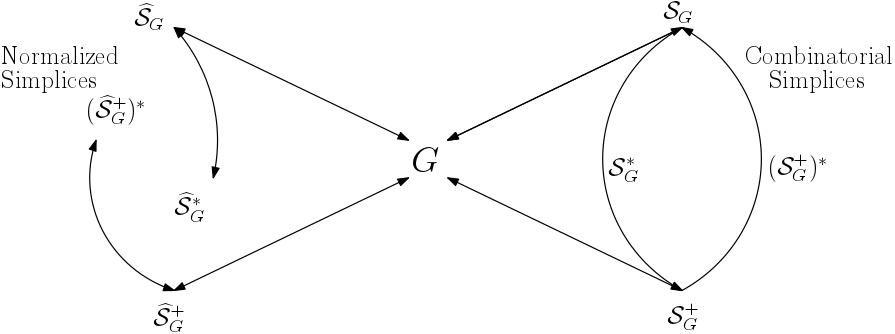
\includegraphics[scale=0.4]{correspondence}
	\caption{An illustration of the various objects and relationships in the graph-simplex correspondence. The combinatorial simplices sit to the right of $G$, while the normalized simplices sit to the left. We see that  $\splx_G$ and $\splx_G^+$ are duals to one another. The normalized simplices,  on the other hand, are not each others duals as exemplied by the discontinuity of the arrows. The arrows between $G$ and each of its simplices demonstrates how the relationship is formed.  }
	\label{fig:correspondence}
\end{figure}

We provide a self-contained treatise of the graph-simplex correspondence, accessible  to those with only  basic knowledge of linear algebra and  graph theory. We include Fiedler's main results  on the topic, as well those newly discovered results of Devriendt and Van Mieghem~\cite{devriendt2018simplex}. We also expand on these results in several ways,  enumerated  below. 




\begin{itemize}
	\item {\bf Introduction of the Dual Simplex.} First, although at first seemingly unrelated to the correspondence itself, we provide a  novel mathematical treatment of an object we call the ``dual simplex'' of a given simplex. This object was remarked upon by Fiedler in his 2011 book~\cite{fiedler2011matrices}, but he did not investigate its properties. We present several general properties of  the dual simplex and use it to frame graph-simplex correspondence, especially of the normalized Laplacian. 
	\item {\bf Extension of Correspondence to the Normalized Laplacian. }While Fiedler (implicitly) and Devriendt and Van Mieghem (explicitly) studied the correspondence by means of the combinatorial Laplacian of a graph, we expand the correspondence to the ``normalized'' Laplacian.  This matrix also describes the complete structure of the graph, but is more intimately related to several of its features, such as describing random walk dynamics~\cite{chung1997spectral}. We introduce this new mapping  along with the original in Section~\ref{sec:bijection_graphs_simplices}. 
	We then study the properties of the simplex associated to the normalized Laplacian, which we term the ``normalized'' simplex.   We refer  the reader to Figure~\ref{fig:correspondence}. 
	\item {\bf First analysis of the Normalized Simplex. } With regards to the normalized simplex, in Section~\ref{sec:Sn_G} we investigate its mathematical properties. This proves a more challenging task   than  in  the case of the combinatorial simplex because, as we will show, the inverse normalized simplex  is \emph{not} the dual of the normalized  simplex in general.
	\item {\bf New Graph Equations and Inequalities.} 
	\begin{figure}
		\centering
		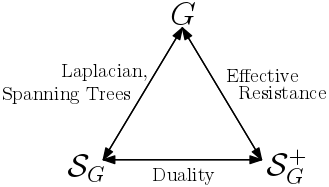
\includegraphics[scale=0.5]{property_triangle}
		\caption{A visualization of how the correspondence can be used to apply graph-theoretic knowledge to the geometry  of the simplices and vice versa. For example, leveraging that the geometry of $\splx_G^+$ is intimately related to the effective resistances of $G$ and relating the equations of $\splx_G^+$  to those of $\splx_G$ via duality allows us  to, say, express equations of spanning trees in terms of effective resistances.  }
		\label{fig:property_triangle}
	\end{figure}
	
	Combining Fiedler's block matrix approach with that of Devriendt and Van Mieghem, we are able to uncover several new relationships. 
	
	For example, between the  entries of the Laplacian and the total  weight of spanning trees in  the graph (Lemma~\ref{lem:L(i,i)_trees}), between the vertices of $\splx_G$  and the volumes of its faces (Equation~\eqref{eq:||sv_i||_vol}), between the Laplacian and the volumes of facets of $\splx$ (Equation~\eqref{eq:vol/vol})). We also  obtain new inequalities pertaining to the spanning trees of $G$ (Lemma~\ref{lem:tree_inequalities}). 
	
	
	
	\item {\bf Link between Resistive Polytope and $\splx_G^+$.} We also uncover a link between the simplex of a graph and a geometric  object related to the effective resistance of the graph, which we call the ``effective polytope''. It seems that the existence of this object has been previously acknowledged (e.g., ~\cite{shayanNotes}), but never rigorously studied. This material appears in Section~\ref{sec:resistive_polytope}. 
	\item {\bf Algorithmic Analysis of the Correspondence.} Perhaps most significantly, we initiate the study of the algorithmic foundations of the correspondence (Chapter~\ref{chap:algorithmics}). This entails three distinct aspects. 
	\begin{enumerate}
		\item {\bf Consequences for Computational Complexity.}	We explore several consequences for computational  complexity.  Owing to the ubiquity of graphs in theory and application, the complexity classes of many graph-theoretic problems are  well established (e.g., computing maximum-cuts and independent sets are ``hard'', while spanning trees are ``easy'', etc.) If, via the correspondence, such problems have analogues in the simplex then this has implications concerning the difficulty of these geometric problems. Moreover, while the analogues problems in the simplex domain may have known to be easy or hard  in general convex polytopes, understanding the complexity in (hyperacute) simplices may yield an improved understanding of the hardness ``threshold'' for such problems. 
		\item {\bf Lower Bounds on Computing the Correspondence.} We then explore the natural question of whether various aspects of the correspondence can be computed efficiently. For example, given $G$ how quickly can we compute $\splx_G$ or $\splx_G^+$ efficiently? What about computing $\splx_G$ given $\splx_G^+$, or vice  versa? Our results in this  space are mostly negative; transitioning between many of these objects require time no less than that required to perform an eigendecomposition of a Laplacian matrix. 
		This is perhaps to be expected given that the mapping is based on the eigendecomposition of the Laplacian matrix. 
		However, we emphasize is it not immediate; while the mapping relies on the eigendecomposition, it uses the relations between the eigenvalues and eigenvectors. It is a priori  feasible that the relationships are computable  more quickly than the eigenvalues and eigenvectors  themselves. 
		\item {\bf Approximations of Various Objects.} Finally, we explore several approximations. Given that  the simplex of a graph with $n$ vertices lives in $\R^{n-1}$---a high dimensional  space---we might hope that we can ``approximately'' embed it  in  lower dimensions. We explore this possibility in Section~\ref{sec:algorithmics_JL}. Owing to the lower bounds achieved on the ``precise'' mappings between various objects mentioned above, we might hope that we can approximate several of these mappings. This is explored in Section~\ref{sec:algorithmics_approximations}. 
		Instead of purely geometric approximations, we might also wonder what happens to the correspondence when we approximate the Laplacian with another. 
	\end{enumerate}

\end{itemize}

\section{Organization}
\label{sec:intro_organization}

The rest of the thesis will be  organized as follows. Chapter~\ref{chap:background} will present the relevant background material in the areas of linear algebra, spectral graph theory, and simplex  geometry. Here we will also define and make some preliminary explorations of the dual simplex. The  background material  of Sections~\ref{sec:background_general}, \ref{sec:background_linear},  and \ref{sec:background_laplacian} is quite standard; the reader familiar with  these subject areas should  be able to skip  them without too much trouble. We  encourage all readers to peruse Section~\ref{sec:background_simplices} because, for one, the field  of simplex geometry is  less  well  studied  in general than the others and secondly, as stated above, we provide a novel treatment of  the dual simplex. Chapter~\ref{chap:correspondence} then presents the  graph  simplex correspondence and explores its  basic mathematical properties.  









     

  	
